\documentclass{../source/Experiment}

\major{信息工程}
\name{}
\title{模拟锁相环与 FM \& FSK 解调}
\expname{模拟锁相环与 FM \& FSK 解调}
\stuid{}
\college{信息与电子工程学院}
\date{\today}
\lab{东4-319}
\course{通信原理实验}
\instructor{金向东、龚淑君}
\grades{}
\exptype{验证性实验}
\partner{}
\begin{document}
\makecover
\makeheader
\section{实验目的和要求}
 (1) 掌握锁相环基本工作原理

(2) 掌握由锁相环实现 FM\_FSK 解调工作原理

(3) 对锁相环主要性能指标进行测量

(4) 对 FM\_FSK 解调相关参数进行测量分析


\section{实验原理}
锁相环是一种相位负反馈系统,当系统锁定时,锁相环电路中鉴相器的两个输入信号,一个来自外部输入,另一个来自压控振荡器,它们的频率相等,相位存在一定的稳态误差。因此锁相环电路具有良好的窄带载波跟踪性能和宽带调制跟踪性能,广泛应用于锁相解调、载波提取与位同步恢复以及频率合成技术中。

\subsection{模拟锁相环的主要性能指标}

(1) 鉴相器的鉴频鉴相特性

(2) 压控振荡器的压控特性

(3) 环路滤波器的滤波特性

(4) 环路的跟踪和捕捉特性
\subsection{基本的模拟锁相环电路结构}
\begin{figure}[H]
    \centering
    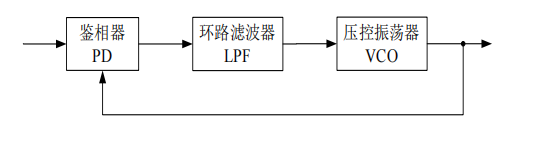
\includegraphics[width = 0.5\textwidth]{lab4/2.png}
    \caption{锁相环电路结构}
\end{figure}



\subsection{FM\_FSK 解调}
锁相环电路的一个重要应用就是鉴频,可以用来进行FM\_FSK解调。若锁相环的输入信号是FM或FSK调频信号,频率受控于调制信号。
当锁相环路锁定时,压控振荡器的输出信号频率将跟随输入信号频率,因此可以从环路滤波器的输出信号中得到调制解调信号。

\section{实验电路分析}
实验电路电路采用NE654集成锁相环芯片,NE654的最高工作频率可达50MHz,芯片内部主要有限幅器、相位比较
器(鉴相器)、压控振荡器、放大器、直流恢复电路和施密特触发器组成。环路滤波器由芯片内置电阻和外接在4脚、5脚的电容构成。相位
比较器采用双平衡乘法器结构,前置的限幅放大器,改善对寄生调幅的抑制作用。在2脚外接滑动变阻器,改变2脚的偏置电流,可以调节相
位比较器的增益,从而改变整个锁相环路的增益。压控振荡器由射极耦合谐振器构成,它的自由振荡频率为

$f_0 = \dfrac{1}{22R_C(C_1 + C_S)}$。

其中, $R_C$ 的值为100欧,$C_1$是外接在12、13脚之间的电容,$C_S$ 是寄生电容。通过调整电容$C_1$数值,可以改变振荡器的自由振荡频率。

\begin{figure}[H]
    \centering
    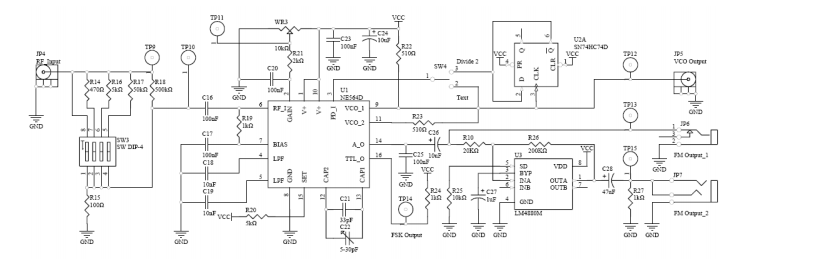
\includegraphics[width = 0.5\textwidth]{lab4/1.png}
    \caption{锁相环FM\_FSK解调电路}
\end{figure}

实验电路如上图所示,主要由输入端的可调衰减器,锁相环电路(U1),二分频电路(U2)和音频功放(U3)组成。进行FM\_FSK解调
时,调制信号从6脚输入,经过限幅器,消除寄生调幅,送到相位比较器的一个输入端。压控振荡器产生的信号由3脚反馈回相位比较器。通
过调节12、13脚的可变电容,使环路锁定。若是FM解调,则相位比较器输出的信号经过恒流源差分放大器放大,再经过直流恢复电路,在14
脚得到FM解调输出,再由LM4880音频放大器放大,得到FM解调音频信号。若是FSK解调,信号经过放大器放大后,一路送到施密特触发器的
输入端,另外一路送到直流恢复电路,由14脚外接的电容构成的低通滤波器滤波,产生一直流电压,送到施密特触发器的另外一个输入端作
为基准电压,进行比较判断,将FSK解调信号的高低电平解调出来。因此,实验电路中,$\rm TP_{13}$、$\rm TP_{15}$分别是音频放大
前后的FM解调输出信号。$\rm TP_{14}$是FSK解调输出信号。

另外,由开关控制选择,锁相环里的压控振荡器输出可以经过D触发器二分频电路后再输入鉴相器,这样就构成了一个倍频电路。倍频信号由压控振荡器输出端$ \rm TP_{12}$得到。



\section{实验设备}
\begin{enumerate}
    \item 实验办No01 \, 1块
    \item 信号源1台
    \item 双踪示波器1台
    \item 频谱分析仪(含TG)1台
    \item 万用表1台
\end{enumerate}

\section{实验数据与结果分析}
\subsection{锁相环同步带、捕捉带的测量}

高频信号源与电路板连接,从$\rm JP_4$端输入频率为10.7MHz,幅度为500mV的正弦波信号。将$\rm TP_9$、$\rm TP_{12}$端口
信号接入双踪示波器。以输入信号作为示波器双踪显示波形的触发源,若两个通道的信号都能同步稳定的显示,则表明锁相环路锁定。
若没能锁定,则微调输入信号频率。

在环路锁定的情况下,持续提高输入信号的频率,直到环路刚刚失锁,记此时的输入信号频率为 $f_{H1}$ ;再慢慢降低输入信号频
率,直到环路刚刚重新锁定,记此时的输入信号频率为$f_{H2}$ ;继续降低输入信号频率,直到环路刚刚再次失锁,记此时的输入信号频率为 $f_{L1}$ ;再次慢慢提高输入信号频率,直到环路又一次刚刚锁定,记此时的输入信号频率为 $f_{L2}$ 。


经过测量得到$ f_{H1}=11.09MHz $,
$ f_{H2}=10.750MHz $,$ f_{L1}=10.470MHz $,$ f_{L2}=10.120MHz $,因此可以通过公式计算出同步带和捕捉带。

同步带=$f_{H1}-f_{L1}$=0.970MHz

捕捉带=$f_{H2}-f_{L2}$=0.280MHz

\subsection{FM\_FSK 解调 }
\subsubsection{FM 解调}

用高频信号源输入一载波频率10.7MHz,信号幅度0dBm,调制信号为1kHz的正弦信号,调制频偏为75kHz的FM信号,用示波器观察
解调输出信号(TP13)。改变输入信号的频偏值在10kHz-80kHz之间以10kHz步进变化,用示波器观察解调输出信号的幅度变化。
列表记录,并画出鉴频曲线。
表格记录如下:
\begin{table}[H]
    \centering
    \begin{tabular}{|c|c|}
        \hline
        输入信号频偏值 & 解调输出信号幅度 \\ \hline
        10kHz          & 没有解调信号     \\ \hline
        20kHz          & 14.4mV           \\ \hline
        30kHz          & 17.2mV           \\ \hline
        40kHz          & 22.4mV           \\ \hline
        50kHz          & 26.4mV           \\ \hline
        60kHz          & 31.4mV           \\ \hline
        70kHz          & 34.2mV           \\ \hline
        80kHz          & 38.4mV           \\ \hline
    \end{tabular}
\end{table}

\begin{figure}[H]
    \centering
    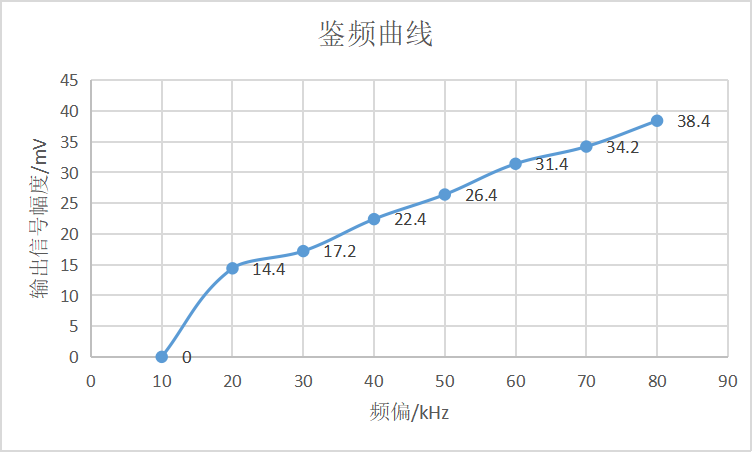
\includegraphics[width = 0.5\textwidth]{lab4/图片1.png}
    \caption{鉴频曲线}
\end{figure}

从图中可以看出频偏值增大时,解调信号也增大,并且可以看出在FM调制中,输出信号幅值和频偏值呈线性关系。
\subsubsection{FSK 解调}

用高频信号源输入一载波频率10.7MHz,信号幅度0dBm,调制信号为频率1kHz的方波信号,调制频偏为75KHz的FSK信号,示波器
观测解调输出信号(TP14)。逐渐减小输入信号的幅度,观察解调输出信号,直到出现没有解调信号输出的情况,此时的输入信
号幅度记为解调灵敏度,请作记录。

实验得输入信号幅度为-27.5dBm时没有解调输出信号,此即为解调灵敏度。
。

\section{思考题}
\subsection{阐述模拟锁相环工作的基本原理 }

基本的锁相环电路主要由三部分组成:鉴相器、环路滤波器和压控振荡器。

鉴相器对它的两个输入信号相位作相减操作,并将相位差值转换成电压输出。此电压正比与两输入信号的相位差,关系如下式所示:

$v_d(t) = A_d\varphi_e (t)$

$A_d$是鉴相灵敏度,线性关系只有在$\varphi_e(t)$的一定范围内满足,此范围称为线性鉴相范围。

环路滤波器滤除鉴相器输出电压中的高频成分和噪声,输出平均分量,作为压控振荡器的控制电压。因此,环路滤波器为低通滤波器,在锁相环路中主要关注的性能指标包括滤波带宽和增益。

压控振荡器是一个频率受控器件,频率与控制电压之间的关系如下式所示:

$\omega_c(t) = \omega_o + A_o v_c(t)$

其中,$\omega_o$是当控制电压为零时,压控振荡器的自由振荡频率,$A_o$是压控灵敏度。

当构成闭环系统后,随着环路的反馈控制,鉴相器两输入信号之间的频率差越来越小,当频率差为零时,环路锁定,进入稳定状态。此
时系统具有一个稳态相位误差,产生的控制电压控制压控振荡器的频率,使它与输入信号的频率相等。这个相位误差与环路增益有关,增益越大,相位差越小。

锁相环还具有两个特性:跟踪和捕捉。处于锁定状态的电路,当输入信号的频率或相位发生变化,鉴相器输出也随之发生变化,环路滤
波器的输出控制压控振荡器,使它的频率能跟随输入信号的频率变化,则环路仍处于锁相状态,这一过程称为跟踪。环路通过跟踪过程
能够保持环路锁定的最大输入频差,称为同步带。

捕捉是指环路在失锁的状态下,通过自身电路的调节进入锁定状态的过程。捕捉包括频率牵引和快捕两个过程。当鉴相器两输入信号的
频率差太大时,鉴相器输出的相位差信号频率很高,几乎都被低通环路滤波器滤除,也就没有信号去控制压控振荡器,不可能捕捉。而
当输入频差没有那么大,处于能捕捉的频率范围,则环路滤波器就有一定的输出电压,控制振荡器频率发生变化,使频率差进一步减
小。此过程就是频率牵引的过程。当频率差小到一定程度,使得压控振荡器的控制电压在正弦变化的一个周期内就能将频率捕捉,使环
路锁定,这就称为快捕。因此,环路通过频率牵引和快捕,最终能锁定的最大输入信号频率差就是捕捉带。

\subsection{环路同步带和捕捉带的概念是什么?}
环路通过跟踪过程
保持环路锁定的最大输入频差,称为同步带。

因此,环路通过频率牵引和快捕,最终能锁定的最大输入信号频率差就是捕捉带。
\subsection{FM\_FSK 调制信号频偏对解调的影响是什么?}
频偏越大解调信号的幅度越大,并且一定范围内呈线性关系。
\subsection{锁相环鉴频有何优缺点?}
当失去基准频率,输出频率跳回振荡器本身的频率;并且当进行频率调整的时候,输出频率会产生抖动,频差越大,抖动会越大,不利于某些领域的应用。
\end{document}